\documentclass{report}
\usepackage[T1]{fontenc}
\usepackage{color}
\usepackage{amssymb}
\usepackage{pdfpages}
\usepackage{amsmath}
\usepackage{eurosym}
\usepackage{graphicx}
\usepackage{textcomp}
\usepackage{listings}
\usepackage{epigraph}
\usepackage{setspace}
\usepackage{array}
\usepackage{gensymb}
\usepackage{tikz}
\usepackage[some]{background}
\usepackage{geometry}
\usepackage[english]{babel}


\begin{document}
\renewcommand{\chaptername}{Partie}
\renewcommand{\thechapter}{\Roman{chapter}}

%\usepackage{lmodern}
%\usepackage{xspace}
%\usepackage{hyperref}

\definecolor{sup_strip_color}{rgb}{0.80,0.80,0.80}
\definecolor{inf_strip_color}{rgb}{0.00,0.00,0.00}

\DeclareFixedFont{\bigsf}{T1}{phv}{b}{n}{0.8cm}

\makeatletter                       
\def\printauthor{%                  
    {{\large \@author}}}              
\makeatother

\author{Zohour \textsc{Abouakil} ~\\ Sofia \textsc{Boutahar} ~\\ David \textsc{Courtinot} ~\\ Xiaowen \textsc{Ji} ~\\ Fabien \textsc{Sauce}}

\begin{titlepage}

\newgeometry{left=1cm,right=4cm,bottom=0cm}
\begin{tikzpicture}[overlay,remember picture]
% the black stripe with the title
\node[
  fill=inf_strip_color,
  anchor=north west,
  text width=\paperwidth,
  text height=2cm,
  text depth=2cm,
  inner xsep=1cm,
  font=\color{white}\bigsf 
  ] 
 at ([yshift=-2.5cm]current page.north west) (blackrect) {Design review - Iteration 1 - Version 2};
% the khaki stripe
\path[fill=sup_strip_color] 
  (blackrect.north west) rectangle ++(\paperwidth,2.5cm);
\end{tikzpicture}

\vspace*{4.5cm}

\noindent
\begin{minipage}{0.35\linewidth}
    \begin{flushright}
        \printauthor
    \end{flushright}
\end{minipage} \hspace{15pt}
%
\begin{minipage}{0.02\linewidth}
    \rule{1pt}{175pt}
\end{minipage} \hspace{-10pt}
%
\begin{minipage}{0.6\linewidth}
\vspace{5pt}
\newenvironment{test}{\begin{center}}{\end{center}}
\hspace{10pt}
\begin{minipage}{\linewidth} 
\textbf{Reference :} model-checking.design ~\\
January $30^{th}$ 2015
\end{minipage}
\end{minipage}

\vspace{8cm}
\begin{minipage}{0.20\linewidth}
    \begin{flushright}
       
        \begin{tabular}{ll}
	 \textit{Signatures} & \\
            & \textbf{Quality responsible :} \\
            & \textbf{Clients :} \\
        \end{tabular}
    \end{flushright}
\end{minipage}

\end{titlepage}
\restoregeometry
\tableofcontents
\newgeometry{left=2.1cm,right=2.1cm}
\chapter{AST and CFG representations}

\paragraph{}
\hspace{4mm}\textnormal{After studying the Clang API, we came to the conclusion that the AST is a much more low-level representation of the programme than the CFG. 
Indeed, the atom for a CFG is what is generally called a \textit{statement} whereas the simplest instruction
gives an AST representation composed of multiple nodes. We also found it difficult to handle the parsing and the linking of the graph nodes at the same time.
Thus, we have chosen to transform the AST into a series of higher-level objects than the original nodes, which will be converted
in nodes of the CFG or supernodes containing a subgraph.}

\section{Intermediate representation of the Clang AST}

\subsection{Parsing the Clang AST file}

\paragraph{}
\hspace{4mm}\textnormal{At first, we have considered using XML parsing libraries to parse the XML version of the Clang AST. However, 
this type of output is no longer supported by the newest versions of the Clang compiler and all the existing tools
provide partial support at best. Hence, we decided using the regular AST file and parse it line by line 
with a custom parser.}

\paragraph{}
\hspace{4mm}\textnormal{We have identified three main kinds of nodes in the AST. Each one is associated to a specific class which extends ASTNode :}

\vspace{4mm}
\begin{itemize}
\item nodes consisting in an type name, an id, a code pointer pointing the relevant lines of the code and some
metadata that depend on the type of the node. These are represented by the ConcreteASTNode class.\vspace{1mm}
\item < < <NULL> > > children, represented by the NullASTNode class.\vspace{1mm}
\item other kind of nodes, prior to class declaration for example. These are represented by OtherASTNode.\vspace{1mm}
\end{itemize}

\begin{center}
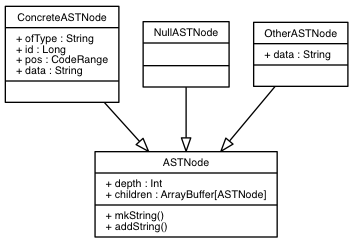
\includegraphics[scale=0.8]{data/ASTNode.png}
~\\~\\Figure I.1 - Inheritance relationships between the classes used to represent the AST
\end{center}

\paragraph{}
\hspace{4mm}\textnormal{The file will be parsed and converted in a tree data-structure which nodes are of type ASTNode. The ASTNode objects
will then be converted in Stmt or Decl accordingly to the class hierarchy we present in the next part.}

\subsection{From ASTNode to ProgramNode}

\subsubsection{Decl class hierarchy}

\paragraph{}
\hspace{4mm}\textnormal{For the Decl part, we did not have too much trouble and just had to associate each high-level Clang Decl class to a Scala class extending
our Decl class.}

\begin{center}
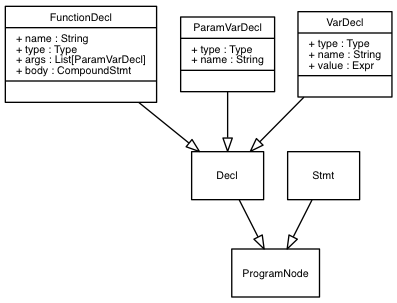
\includegraphics[scale=0.8]{data/decl.png}
~\\~\\Figure I.2 - Class diagram of the imperative part of Decl
\end{center}

\subsubsection{Stmt part}

\paragraph{}
\hspace{4mm}\textnormal{For this first iteration, we have decided to skip the C++ object oriented part in order to focus exclusively 
on the imperative part. Inspired by the Clang API, we came up with the following class diagram :}

\begin{center}
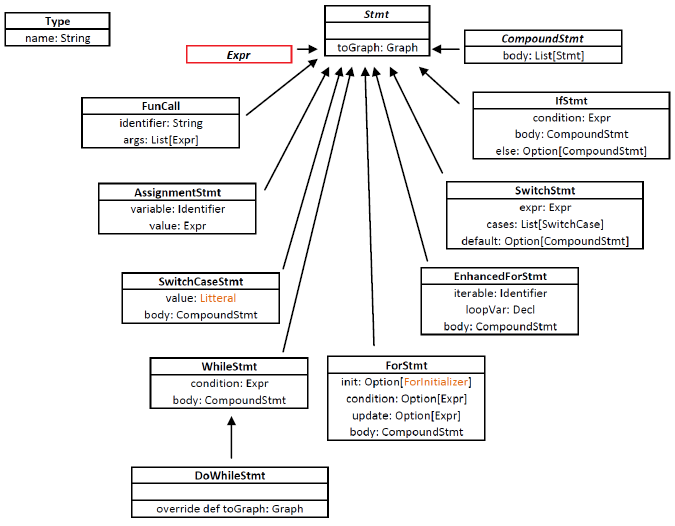
\includegraphics[scale=0.9]{data/stmt.png}
~\\~\\Figure I.3 - Class diagram of the imperative part of Stmt
\end{center}

\paragraph{}
\hspace{4mm}\textnormal{Note that our model does not strictly represent a C$++$ code. For example, we do not prevent a \textit{if} to contain the instruction \textit{break}
(among other inaccuracies ...). We felt that this kind of refinement would unnecessarily complicate the task without adding anything more to the CFG analysis. 
Since the code is already checked semantically by the Clang compiler and given our future needs, we thought it would be wiser to aim for a simple model.
Moreover, some classes have not been totally defined in the previous diagram because we deliberately chose to represent them apart on 
the diagram below. Finally, other classes were not represented (BreakStmt, ContinueStmt for a better readability).}

\begin{center}
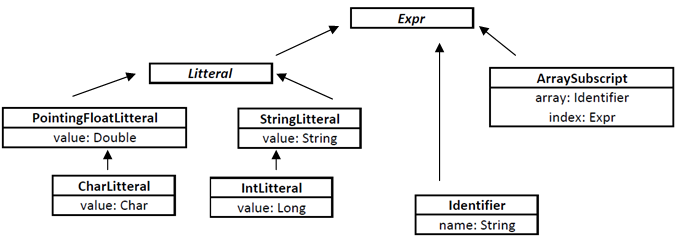
\includegraphics[scale=0.8]{data/expr1.png}
~\\~\\Figure I.4 - Partial class diagram of the \textbf{Expr} part
\end{center}

\paragraph{}
\hspace{4mm}\textnormal{Finally, we present a more complete diagram for Expr even though we still do not know if we will keep it that way,
its complexity being considered superfluous for the nature of the algorithms we will use on these structures.}

\begin{center}
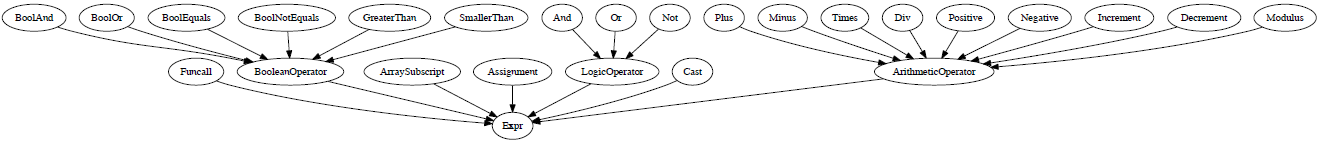
\includegraphics[scale=0.5]{data/expr2.png}
~\\~\\Figure I.5 - Class diagram heavier (still incomplete) for the \textbf{Expr} part
\end{center}

\subsubsection{Important notes}

\vspace{4mm}
\begin{itemize}
\item to accuratelys represent the CFG of our input programs, we must take into account the fail-fast mechanism in the evaluation of boolean conjunctions/disjunctions.
The importance of this mechanism for our project is illustrated in the figure below.\vspace{1mm}
\item however, since the evaluation's order of the expressions is not completely specified specified in C++ (unlike Java which evaluates from left to right),
we will limit these considerations to simple expressions. Therefore we will not take care of expressions (boolean or not) containing 
sub-expressions side effect (increment, assignments...).\vspace{1mm}
\end{itemize}

\begin{center}
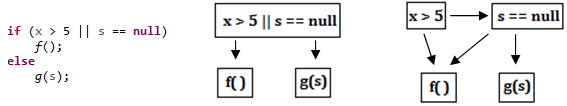
\includegraphics[scale=0.85]{data/fail-fast.png}
~\\~\\Figure I.6 - On the left the considerate code. On the center, we didn't take into account the fail-fast for the CFG, and finally on the right we consider the fail-fast
\end{center}

\paragraph{}
\hspace{4mm}\textnormal{As shown in the figure above, if we try to
assert the property \textit {<< variable s is always initialized when g(s) is called >>}, the first CFG will not allow us to conclude
(or it will conclude \textbf {true}, erroneously) while the second allows us
to state that there are executions, according to the value of x,
where $g$ is called with an uninitialized parameter
(assuming that the left son is always a successful test and the right son is a failed test).}

\paragraph{}
\hspace{4mm}\textnormal{Another important thing to mention is that at the beginning, we had a mix of regular classes with
var/val members and case classes. Moreover, we were using <<var>> immutable lists (class List) for building
incrementally some collections as the list of statements in a compound statement. However, it would imply to append at the end
because otherwise, the list would have been to be reversed each time needed. Thereforce, we have created a simple wrapper of ArrayBuffer,
that hides all the ArrayBuffer definitions except $+=$, and otherwise behaves as an immutable List. Same thing was done with
a wrapper of a mutable HashMap (for storing declaration by their name for example). This enables to use 
a more functional programming style while being efficient.}

\paragraph{}
\hspace{4mm}\textnormal{Finally, we chose to make all the classes as case-classes to enable the powerful Scala pattern-matching.
Hence, it appeared a more flexible and clever conception to separate the Stmt/Decl classes from their 
actual equivalent in the code, which is a ProgramNode. The ProgramNode contains the information of the position
of the Stmt/Decl in the code thanks to the CodeRange class. As we were using case-classes, we could not inherit some constructor from
ProgramNode that would initialize the CodeRange, so we just made the CodeRange optional and added a setter. It seems to be poor design
at first sight but it was the best way to keep the advantages of both the pattern-matching and the factorization of an attribute 
on an abstract superclass.}

\section{AST to CFG}

\paragraph{}
\hspace{4mm}\textnormal{The class GraphNode is used to represent a node of the CFG, it is still not clearly defined as we are missing the operations
required on this class for the model checker. Nevertheless, we can already be sure that a GraphNode will wrap a ProgramNode value (most certainly only certain kind
of ProgramNode such as DeclStmt, Assignment and so on, and never CompoundStmt or classes containing an inner CompoundStmt instance). It will also provide a list
of predecessors and a list of successors so that we can explore the graph.}

\paragraph{}
\hspace{4mm}\textnormal{Finally, we have thought about the problem of the label function. We must be able to labellize many different kinds of nodes
with any kind of predicate. We do not want that adding a new predicate require rewriting the ProgramNode children classes, so we opted for
a Visitor pattern. Thus, adding a new Label will only consist in writing a class extending the Labellizer trait.}

\begin{center}
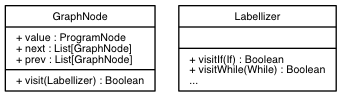
\includegraphics[scale=0.8]{data/CFG.png}
~\\~\\Figure I.7 - CFG class diagram
\end{center}

\chapter{Model checking}

\end{document}
